%%%%%%%%%%%%%%%%%%%%%%%%%%%%%%%%%%%%%%%%%%%%%%%%%%%%%%%%%%%%%%%%%%%%%%%%%%%
%
% Plantilla para un artículo en LaTeX en español.
%
%%%%%%%%%%%%%%%%%%%%%%%%%%%%%%%%%%%%%%%%%%%%%%%%%%%%%%%%%%%%%%%%%%%%%%%%%%%

% Qué tipo de documento estamos por comenzar:
\documentclass[a4paper]{article}
% Esto es para que el LaTeX sepa que el texto está en español:
\usepackage[spanish]{babel}
\selectlanguage{spanish}
% Esto es para poder escribir acentos directamente:
\usepackage[utf8]{inputenc}
\usepackage[T1]{fontenc}
\usepackage{float}


%% Asigna un tamaño a la hoja y los márgenes
\usepackage[a4paper,top=3cm,bottom=2cm,left=3cm,right=3cm,marginparwidth=1.75cm]{geometry}

%% Paquetes de la AMS
\usepackage{amsmath, amsthm, amsfonts}
%% Para añadir archivos con extensión pdf, jpg, png or tif
\usepackage{graphicx}
\usepackage[colorinlistoftodos]{todonotes}
\usepackage[colorlinks=true, allcolors=blue]{hyperref}

%% Primero escribimos el título
\title{M-tree}
\author{Bejar Merma Angel Andres\\
  \small Universidad Nacional de San Agustin\\
  \small abejar@unsa.edu.pe\\
  \small Ciudad de Arequipa
  \date{}
}

%% Después del "preámbulo", podemos empezar el documento

\begin{document}
%% Hay que decirle que incluya el título en el documento
\maketitle

%% Aquí podemos añadir un resumen del trabajo (o del artículo en su caso) 
\begin{abstract}
El objetivo de esta investigación es Describir, implementar la estructura de datos M-Tree.Analizar el funcionamiento de la estructura M-Tree.
\end{abstract}

%% Iniciamos "secciones" que servirán como subtítulos
%% Nota que hay otra manera de añadir acentos
\section{Introducci\'on}

Es una estructura similar al R-tree u B-tree y se construye utilizando una métrica y se basa en la desigualdad triangular
para consultas de rango eficiente y k vecino más próximos (k-NN). Como en cualquier estructura de datos basada en árboles,
M-Tree se compone de nodos y hojas. En cada nodo hay un objeto de datos que lo identifica de forma única y un puntero a
un subárbol donde residen sus hijos. Cada hoja tiene varios objetos de datos. Para cada nodo hay un radio r que define una
esfera en el espacio métrico deseado. Por lo tanto, cada nodo n y hoja l que reside en un nodo en particular N está a una
distancia máxima r de N, y cada nodo n y hoja l con el nodo principal N mantén la distancia\cite{Ciaccia97m-tree:an}\cite{Ciaccia1997IndexingMS}.
\begin{figure}[H]
  \centering
  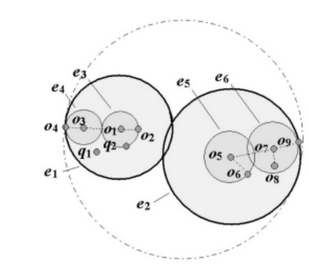
\includegraphics[width=0.6\textwidth]{imagenes/Captura de pantalla de 2021-12-16 00-34-09.png}
   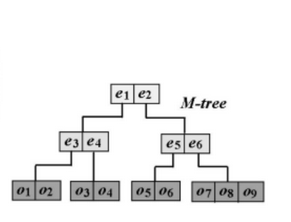
\includegraphics[width=0.6\textwidth]{imagenes/Captura de pantalla de 2021-12-16 00-33-54.png}
  \caption{Visualización del \textbf{mtree} con 9 nodos se muestran en jerarquía de esferas y estructura árbol}
\end{figure}
El árbol M ofrece tres formas diferentes de buscar a través de objetos indexados:

\begin{enumerate}
    \item \textbf{Consulta de rango:}
     Para una consulta de rango, el usuario debe especificar un objeto de consulta como q y un radio de consulta como  r. Entonces el árbol, devuelve todos aquellos objetos indexados o cuya distancia d de q no es mayor que r, es decir, para los cuales d (o, q) <= r.
     
     \item \textbf{consulta K vecinos mas cercanos:}
      Para una consulta de k vecinos más cercanos, el usuario especifica el objeto de consulta q y el número de vecinos k. Entonces, se devuelven k objetos indexados que tienen la distancia mínima d desde q.
      
      \item \textbf{Acceso ordenado:}  El modo de búsqueda de acceso ordenado puede verse como una búsqueda interactiva de vecino más cercano, donde el usuario puede buscar iterativamente el próximo vecino más cercano del objeto de consulta. Para ello, el usuario solo tiene que especificar el objeto de consulta q. Luego, cada vez que el usuario solicita otro objeto, el árbol devuelve el objeto indexado que es el más cercano a q (según la distancia d) entre los que aún no han sido devueltos al usuario\cite{pag}.
\end{enumerate}


\section{Desarrollo}


Esta es una implementación del árbol M, una estructura de datos para encontrar los elementos más similares a un elemento dado.

El árbol M es una implementación basada en Tree enfocado en el   espacio métrico
\url{http://en.wikipedia.org/wiki/Metric_space}, es similar al árbol B.

Implementación basada en el papel
'M-tree: Un método de acceso eficiente para la búsqueda de similitudes en espacios métricos'

Para usar el  MTree solo necesitas pasarle dos cosas:
\begin{itemize}
    \item Un conjunto de objetos para almacenar.
    
    \item Una función de distancia 'd (x, y)' que devuelve un número que establece
qué tan similares son dos objetos.
\end{itemize}

\begin{figure}[H]
  \centering
  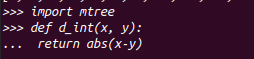
\includegraphics[width=0.5\textwidth]{imagenes/Captura de pantalla de 2021-12-15 23-51-51.png}
  \caption{función distancia}
\end{figure}

\begin{figure}[H]
  \centering
  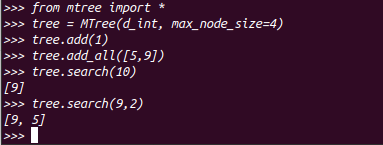
\includegraphics[width=0.6\textwidth]{imagenes/test.png}
  \caption{ejemlplo al ejecutar el programa}
\end{figure}

\noindent
En la figura 2 se  define la función distancia para los números.\\\\En la figura 3
\textbf{Mtree} crea un arbol vacio en la siguiente linea  \textbf{add }agrega el objeto 1 al arbol en la siguiente  \textbf{add all} agrega los objetos 5 y 9,luego \\\\ \textbf{Search} busca el objeto más cercano a 10 que devolvera 9
y la ultima linea busca los dos objetos más cercanos a 9 devolverá 9 y 5.
\\
\\


El tamaño de los nodos (argumento opcional max\_node\_size) tiene una gran influencia en el número de llamadas de la función de distancia ,\textbf{d}.
\\
\\
Los objetos que inserta en el árbol pueden ser cualquier cosa siempre que la función de distancia que proporcione sea capaz de manejarlos correctamente.

La función de distancia \textbf{(d)} debe proporcionarse cuando se crea el árbol. Toma como parámetro dos objetos y devuelve un número que indica qué tan similares son los dos objetos. Cuanto menor sea el número, más similares serán los objetos. El número devuelto puede ser un entero, flotante, o otro Técnicamente, cualquier cosa que se comporte como un número (<, <=,>, ...).

\subsubsection*{La función de distancia DEBE respetar las siguientes propiedades: }

\begin{itemize}
    \item \textbf{d :}Siempre devuelve el mismo valor dados los mismos parámetros
    
    \item \textbf{No ser negativo:} para todo x, y: d (x, y)> = 0,\textbf{ d} nunca debe devolver un valor negativo.  Su función puede ser negativo pero tiene un límite inferior (por ejemplo, nunca devuelve nada inferior a -100),esto se puede solucionar aumentando sistemáticamente el valor de todo el número devuelto (por ejemplo, valor de retorno +100).
    
    
    \item\textbf{ Simetría:} Para todo x, y: d (x, y) = d (y, x) Se debe devolver el mismo valor sin importar el orden de los parámetros.
    
    
    \item\textbf{ Identidad:} Para todo x, y: d (x, y) = 0 significa que x = y.
    
    \item\textbf{ Desigualdad del triángulo:} para todos x, y, z donde d (x, z) <= d (x, y) + d (y, z) La distancia de un punto a un segundo es siempre menor o igual a la distancia de un punto a un intermediario + la distancia desde el intermediario hasta el segundo punto.
    
    

\end{itemize}



Si la función de distancia viola una de estas reglas, el mTree puede devolver resultados erróneos.

Si el mismo objeto se inserta varias veces, el árbol lo considerará como un objeto diferente.





\subsection{Datos}

\begin{figure}[H]
  \centering
  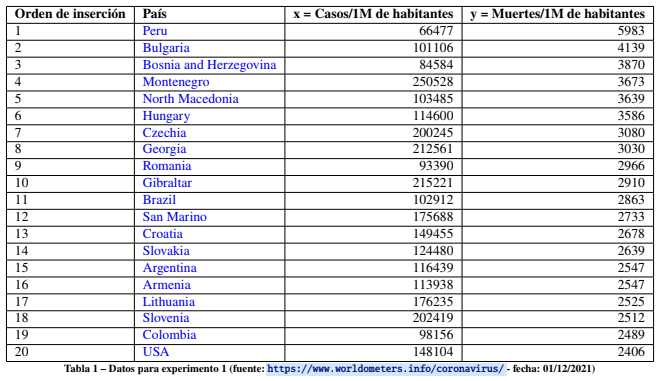
\includegraphics[width=1\textwidth]{imagenes/Captura de pantalla de 2021-12-15 13-58-05.png}
\end{figure}





\subsection{Ejercicios}



\begin{enumerate}
\item  Implemente un M-Tree considerando los procedimientos de inserción y búsqueda.


\item  Inserta conjunto de puntos proporcionado en la tabla 1 en el M-Tree y mostrar gráficamente el estado del árbol después de
insertar:

a) El quinto elemento de la tabla(North Macedonia)
b) El décimo elemento de la tabla(Gibraltar)
c) El último elemento de la tabla(USA)

\item Dada una distancia de 37000, cuantos y cuales son los países más próximos a Perú (mostrar la búsqueda ejecutada y el
resultado en el lenguaje de programación escogido)


\item Cual es el país más próximo de Hungary. (mostrar la búsqueda ejecutada y el resultado en el lenguaje de programación
escogido)


\item Cual de las coordenadas (x o y) es la más determinante en el cálculo de las distancias?


\item Utilice el conjunto de datos proporcionado en la tabla 2 para determinar si existe influencia del orden de inserción de los
datos en el resultado de la búsquedas en términos de los nodos recorridos para generar la respuesta.



\end{enumerate}



\section{Discusión}

Esta implementación es solo de memoria. El árbol no se almacena en el disco. Esto puede ser un problema si los objetos que almacena son grandes (imágenes, sonido, ...). Aunque el árbol en sí reside en la memoria, puede almacenar los objetos que contiene en el disco (o en línea, ...). Por ejemplo, los objetos que pasa al árbol podrían ser rutas a archivos; la función \textbf{d} cargaría los archivos desde el disco para realizar las comparaciones.

Una buena opción para compensar osea  para mantener un buen rendimiento y minimizar el uso de la memoria,  es almacenar en los objetos reales  ,solo  la ruta  a los objetos  reales, así como las características clave que definen a cada dato. 
\\
\\
La función de distancia \textbf{(d)} puede comparar los objetos usando las funciones sin necesidad de acceso al disco. De esa manera, las búsquedas son rápidas (sin acceso al disco) mientras se mantienen los datos en el disco\cite{repositorio}.

\bibliographystyle{abbrv}
\bibliography{sample}

\end{document}